\documentclass[14pt, handout]{beamer}

\usepackage[utf8]{inputenc}
\usepackage[T2A]{fontenc}
\usepackage[russian]{babel}
\usepackage{wrapfig}
\usepackage{caption} 
\usepackage{graphicx}


\usetheme{default}
\usecolortheme{default}


\date{}
\title{Метод и средства передачи данных в реальном времени в программно-конфигурируемых сетях} 
\author{Ермакова Татьяна Ивановна \\ 621}            
\institute{Научный руководитель: \\ к.ф.-м.н., с.н.с. \\ Балашов Василий Викторович}    
\date{}
\setbeamertemplate{frametitle}[default][center]  

\setbeamertemplate{footline}[frame number]

\begin{document}

\begin{frame}[plain]
\titlepage
\end{frame} 




\begin{frame}
\frametitle{Передача данных в системах реального времени}

\begin{itemize}
	\item Требования к качеству передачи данных.
	\item Механизм виртуальных каналов.
	\item Устойчивые пути следования трафика через сеть.
\end{itemize}

\begin{minipage}[0.2\textheight]{\textwidth}
	\begin{columns}[T]

		\begin{column}{0.55\textwidth}
			\begin{itemize}[<+->]
				
				\item Разделение пропускной способности.
				\item Разграничение потоков данных.
			\end{itemize}
		\end{column}
		\begin{column}{0.35\textwidth}
			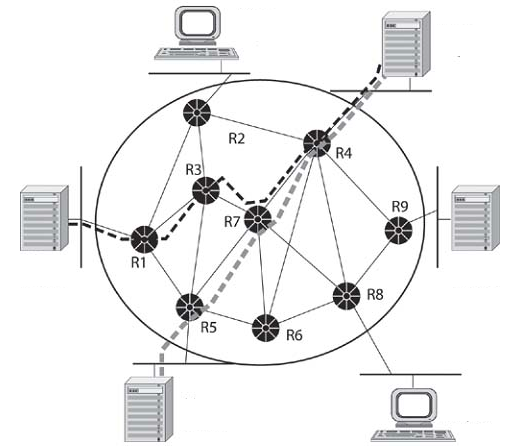
\includegraphics[width=\linewidth]{img/vl.png}
		\end{column}
	\end{columns}
\end{minipage}

\end{frame}



\begin{frame}
\frametitle{Потребность в реконфигурации виртуальных каналов}

\begin{itemize}
	\item Выход из строя элементов ВС РВ.
	\item Смена режима в ходе работы системы.
\end{itemize}

\end{frame}



\begin{frame}
\frametitle{Поддержка реконфигурации виртуальных каналов}

\begin{itemize}
	\item \textbf{AFDX} \\ Отсутствует.
	\item \textbf{FC-AE-ASM-RT} \\ Присутствует возможность заложить несколько статических конфигураций, однако невозможно заложить все множество сбойных режимов.
	\item \textbf{ПКС} \\ Присутствует возможность динамического перераспределения виртуальных каналов.
\end{itemize}

\end{frame}



\begin{frame}
\frametitle{Цель работы}
\begin{center}
	Разработать подход к использованию программно-конфигурируемых сетей в составе вычислительных систем реального времени. В основу подхода должна лечь ранее разработанная автором схема управления потоками данных в ПКС на основе виртуальных каналов.
\end{center}

\end{frame}



\begin{frame}
\frametitle{Поставленные задачи}

\begin{enumerate}
	\item Разработать реализующий подход алгоритм динамической реконфигурации виртуальных каналов в ПКС.
	\item Реализовать предложенный алгоритм в рамках приложения для контроллера ПКС, выполняющего функции мониторинга сети и её реконфигурации при выявлении отказов.
	\item Провести экспериментальное исследование полученного решения по критерию работоспособности в условиях реального времени.
\end{enumerate}

\end{frame}



\begin{frame}
\frametitle{Алгоритм реконфигурации сети}
\begin{center}
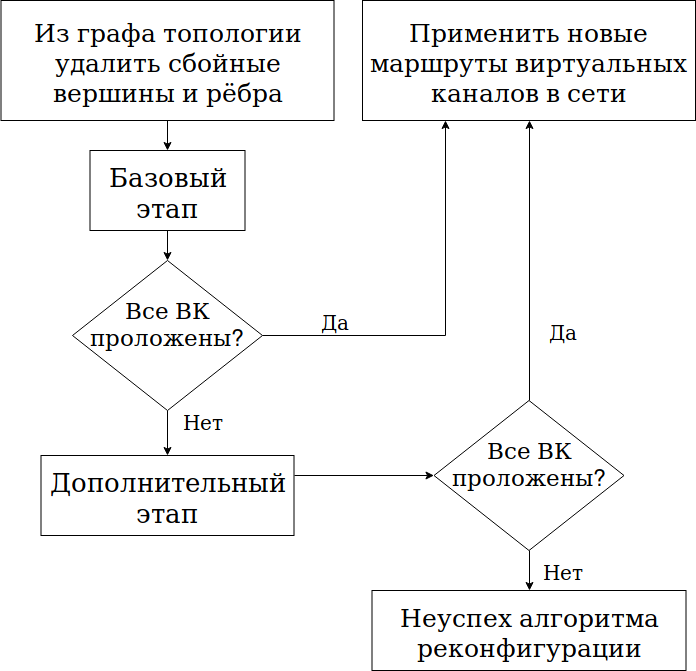
\includegraphics[height=0.85\textheight]{img/alg.png}
\end{center}
\end{frame}


\begin{frame}
\frametitle{Процедуры поиска нового маршрута ВК}
\begin{itemize}
	\item Оценка длины маршрута: \\
		 Вес ребра -- величина, обратная свободной пропускной способности.
	\item Базовый этап: \\
		-- Быстрый поиск. \\
		-- В основе алгоритм Дейкстры от точки отказа к получателю.
	\item Дополнительный этап: \\
		-- Углубленный поиск. \\
		-- В основе алгоритм k-кратчайших путей от отправителя к получателю. \\
		-- Критерий выбора -- совпадение со старым маршрутом.
\end{itemize}

\end{frame}



\begin{frame}
\frametitle{Разработанное приложение для контроллера ПКС}

\begin{center}
	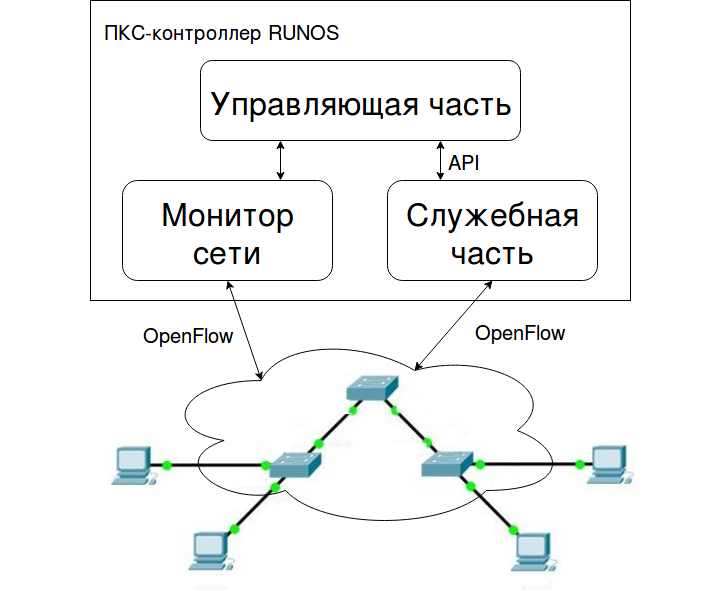
\includegraphics[height=0.8\textheight]{img/netcontrol.png}
\end{center}

\end{frame}


\begin{frame}
\frametitle{Диаграмма основных классов}

\begin{center}
	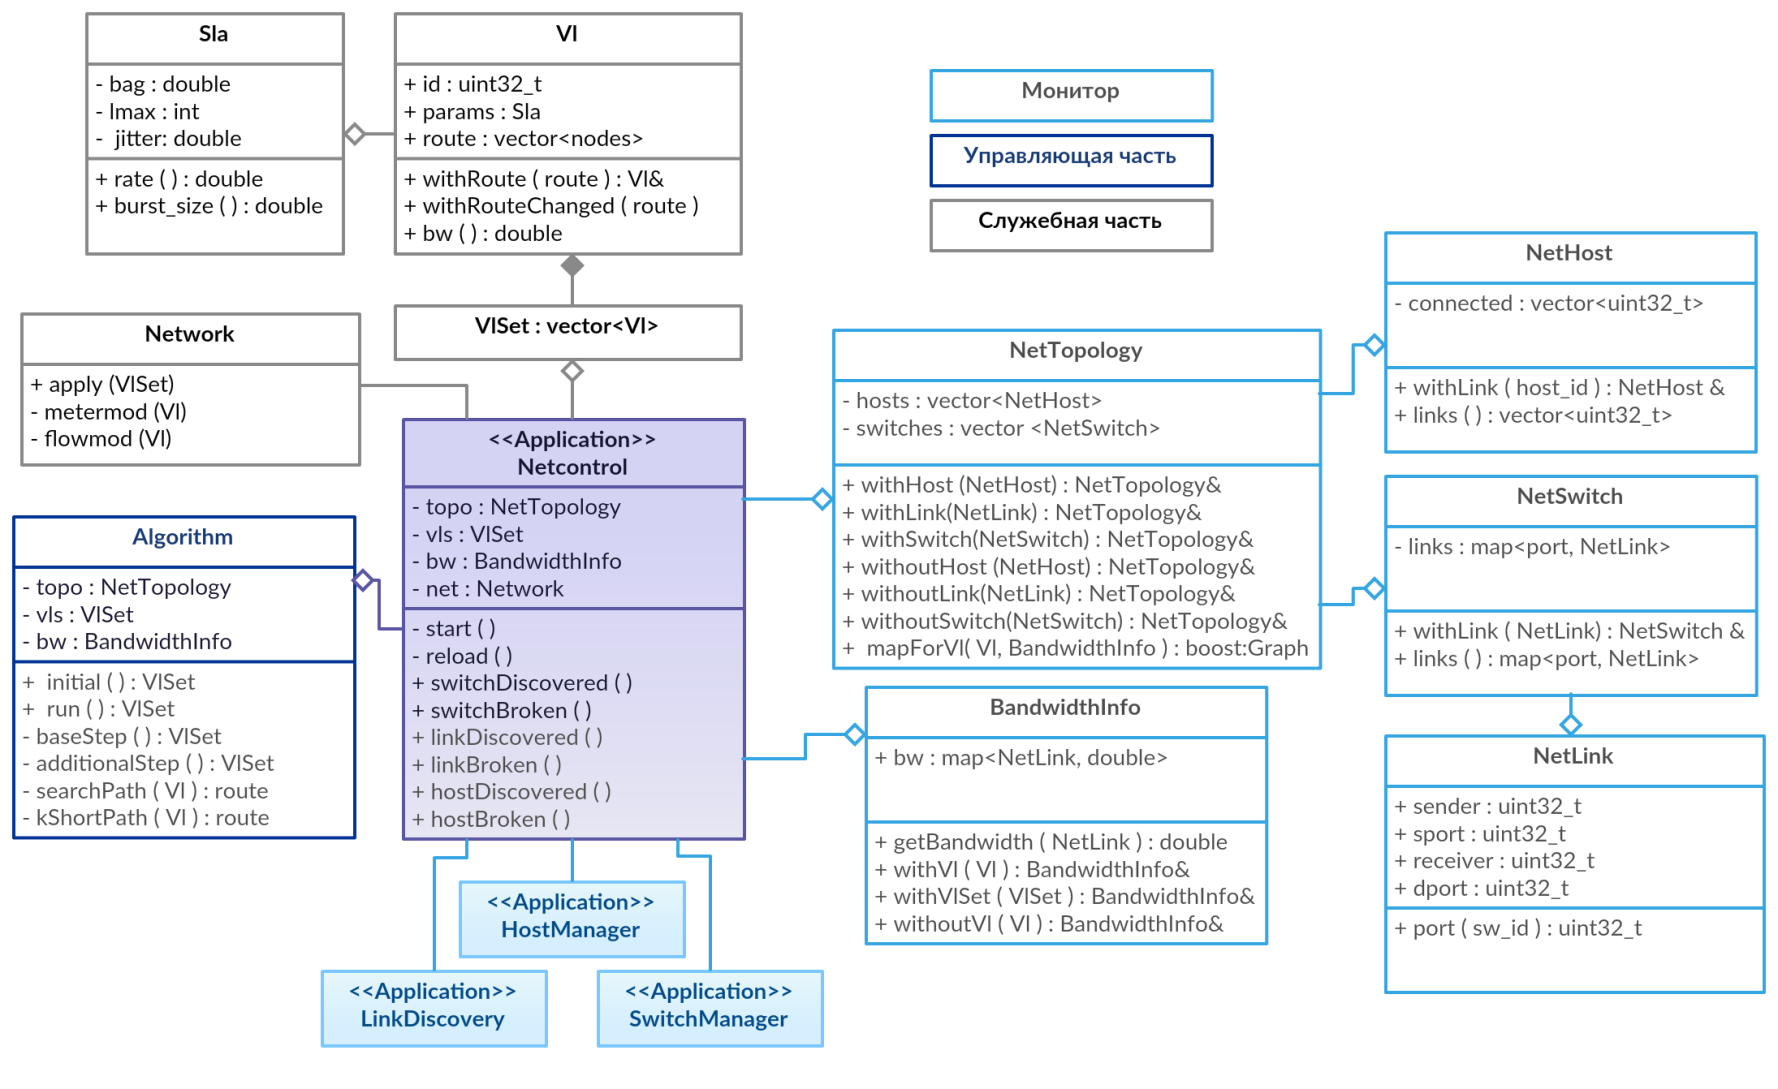
\includegraphics[height=0.78\textheight]{img/classes.png}
\end{center}

\end{frame}


\begin{frame}
\frametitle{Экспериментальное исследование}

Цели:
\begin{itemize}
\item Исследовать характеристики полученного алгоритма на различных классах входных данных; 
\item Подтвердить работоспособность предложенного подхода, включая входящий в него алгоритм, в условиях реального времени.
\end{itemize}

\end{frame}


\begin{frame}
\frametitle{Классы данных}

\begin{itemize}
\item Количество потоков данных: 100.
\item Загруженность сети:\\
	-- 60\% \\
	-- 80\%
\item Распределение виртуальных каналов по пропускным способностям: $$bw = \frac{L_{max}}{BAG}; k = 2 Mbit/c$$
\end{itemize}
\begin{table}[h]
	\small
	\begin{center}
		\begin{tabular}{|c|c|c|c|}
			\hline
			Класс данных& $bw=k$& $bw=2k$& $bw=4k$\\
			\hline
			B1 & 90\% & 7\% & 3\% \\
			\hline
			B2 & 10\% & 80\% & 10\% \\
			\hline
			B3 & 33\% & 34\% & 33\% \\
			\hline
			B4 & 5\% & 15\% & 80\% \\
			\hline
		\end{tabular}
	\end{center}
\end{table}

\end{frame}


\begin{frame}
\frametitle{Топологии сети}

\begin{figure}[h!]
	\vspace{-6ex}
	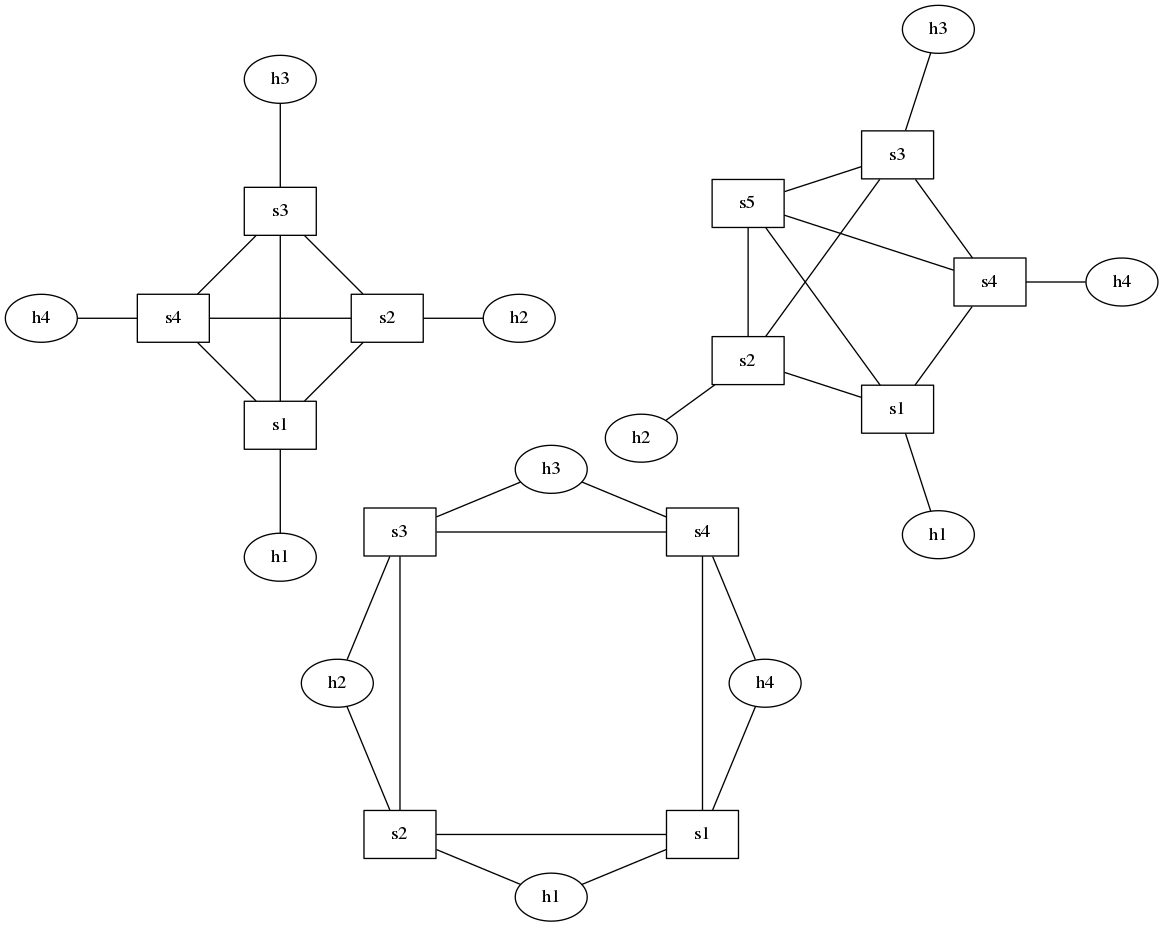
\includegraphics[height=0.95\textheight]{img/topos.png}
\end{figure}

\end{frame}


\begin{frame}
\frametitle{Апробация}

\begin{itemize}
	\item Экспериментальная среда:\\
	-- Mininet. \\
	-- Коммутатор ofsoftswitch13. \\
	-- Контроллер Runos.
	\item Сценарии:\\
	-- Восстановление трафика абонентов при отказах различных элементов сети. \\
	-- Кратный последовательный во времени отказ.
\end{itemize}

\end{frame}

\begin{frame}
\frametitle{Результаты экспериментов}

\begin{minipage}[0.2\textheight]{\textwidth}
	\begin{columns}[T]
		
		\begin{column}{0.5\textwidth}
			\begin{figure}[h!]
				\centering
				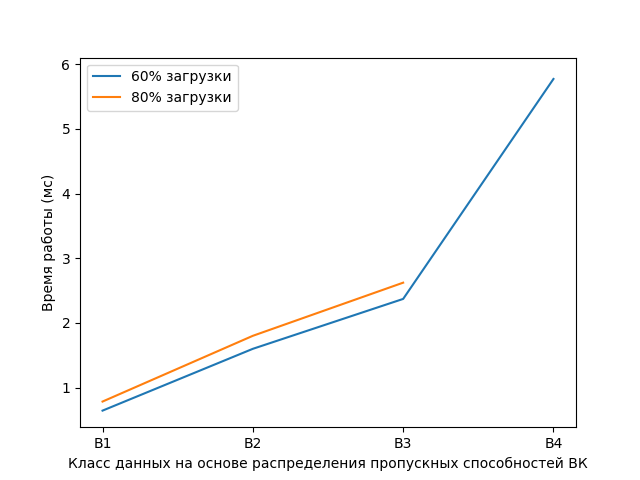
\includegraphics[width=1.0\textwidth]{img/5node_res.png}
				\caption*{Отказ линии в топологии <<Ассиметрия>>.}
			\end{figure}
		\end{column}
		\begin{column}{0.5\textwidth}
			\begin{figure}[h!]
			\centering
			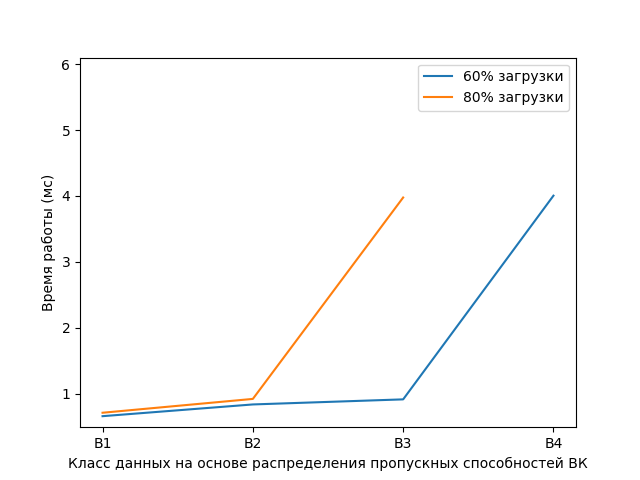
\includegraphics[width=1.0\textwidth]{img/4node_res.png}
			\caption*{Отказ линии в топологии <<Ромб>>.}
		\end{figure}
		\end{column}
	\end{columns}
\end{minipage}


\end{frame}

\begin{frame}
\frametitle{Результаты экспериментов}

\begin{minipage}[0.2\textheight]{\textwidth}
	\begin{columns}[T]
		
		\begin{column}{0.5\textwidth}
			\begin{figure}[h!]
				\centering
				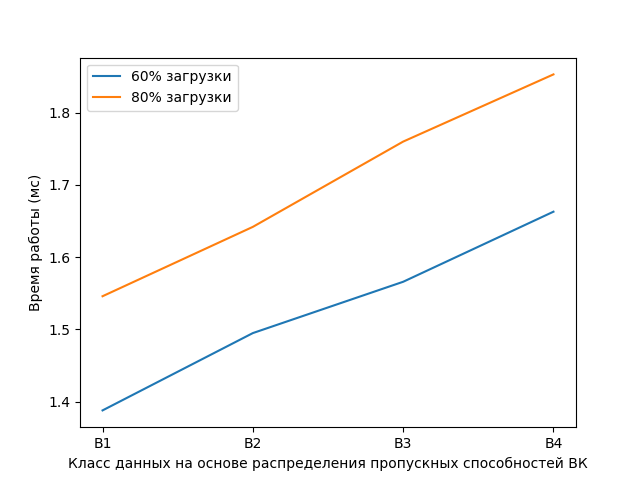
\includegraphics[width=1.0\textwidth]{img/double_res_sw.png}
				\caption*{Отказ коммутатора в топологии <<Двойное резервирование>>.}
			\end{figure}
		\end{column}
		\begin{column}{0.5\textwidth}
			\begin{figure}[h!]
				\centering
				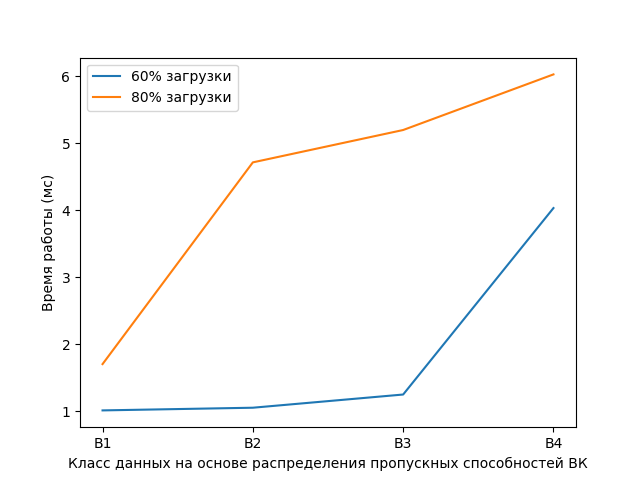
\includegraphics[width=1.0\textwidth]{img/5node_res_sw.png}
				\caption*{Отказ коммутатора в топологии <<Ассиметрия>>.}
			\end{figure}
		\end{column}
	\end{columns}
\end{minipage}


\end{frame}

\begin{frame}
\frametitle{Результаты экспериментов}

\begin{itemize}
	\item Максимальное время работы алгоритма -- 6.028 мс. 
	\item При завершении на базовом этапе -- до 3 мс.
	\item Переход к дополнительному этапу -- 28\% случаев.
	\item Максимальное время, затраченное на процесс реконфигурации, составляет 8 мс.
	\item Параметры качества обслуживания восстанавливаются по завершению реконфигурации.
	\item Максимальное число устраненных последовательных отказов - 4.
\end{itemize}

\end{frame}



\begin{frame}
\frametitle{Результаты работы}

\begin{enumerate}
	\small
	\item Разработан подход к использованию ПКС в составе ВС РВ, основанный на ранее предложенной схеме управления трафиком в ПКС.
	\item Предложен реализующий подход алгоритм динамической реконфигурации систем виртуальных каналов.
	\item Алгоритм реализован в рамках приложения для ПКС-контроллера Runos, осуществляющего функции мониторинга и реконфигурации сети.
	\item С использованием созданного приложения выполнено экспериментальное исследование алгоритма и подхода, демонстрирующее их пригодность для использования в системах реального времени.
\end{enumerate}

\end{frame}




\begin{frame}
\frametitle{Список публикаций}

\begin{itemize}
	\item Балашов В. В., Костенко В. А., Ермакова Т. И. Построение бортовых сетей реального времени на основе технологии ПКС // Моделирование и анализ информационных систем. -- 2019. -- Т. 1, No 26. -- С. 23-38.
	\item Balashov V., Kostenko V., Ermakova T. An SDN-based approach to design of onboard real-time networks // Modern Network Technologies, MoNeTec-2018. -- Moscow, 2018. -- P. 16-22.
\end{itemize}

\end{frame}


\begin{frame}[plain]

\begin{center}
	\LARGE
	Спасибо за внимание!
\end{center}

\end{frame}



\begin{frame}[noframenumbering, plain]
\frametitle{Процедуры поиска нового маршрута ВК}
\begin{itemize}
	\item $S$ -- узел-отправитель.
	\item $R$ -- узел-получатель.
	\item $Node_{S}$ – один из узлов, между которыми прервалась связь, ближний к $S$.
\end{itemize}

Первый вариант процедуры поиска:
\begin{enumerate}
	\item Алгоритм Дейкстры -- путь между $Node_{S}$ и $R$.
	\item Добавить в него путь от $S$ к $Node_{S}$ и удалить циклы.
\end{enumerate}

Второй вариант процедуры поиска:
\begin{enumerate}
	\item Алгоритм k-кратчайших путей -- пути между $S$ и $R$.
	\item Выбрать путь, максимально совпадающий старым маршрутом.
\end{enumerate}

\end{frame}


\begin{frame}[noframenumbering, plain]
\frametitle{Расчет общей загрузки сети}
Для графа сети вес ребра $e$:
$$p_{e} = \sum_{vl}\frac{bw_{vl} \ast k_{vl_e}}{k_{vl}}$$
\begin{itemize}
	\item $bw_{vl}$ -- пропускная способность виртуального канала;
	\item $k_{vl_e}$ -- число кратчайших путей, построенных для ВК через это ребро;
	\item $k_{vl}$ -- число кратчайших путей для  ВК.
\end{itemize}

Общая загрузка сети:
$$p = \max_{e}\frac{p_{e}}{bw_{e}}$$

$bw_{e}$ -- пропускная способность физической линии.

\end{frame}




\end{document}